\documentclass[abstract=on,9pt,twocolumn]{scrartcl}

\usepackage{ucs}
\usepackage[utf8x]{inputenc}
\usepackage[T1]{fontenc}
\usepackage[english]{babel}
\usepackage{datetime}
%\usepackage{multicol}
\usepackage{float}

\usepackage[paper=a4paper,top=2cm,left=1.5cm,right=1.5cm,bottom=2cm,foot=1cm]{geometry}

\usepackage{relsize}%	relative font sizes

\usepackage[retainorgcmds]{IEEEtrantools}%	IEEEeqnarray
\setlength{\IEEEnormaljot}{4\IEEEnormaljot}

\usepackage{graphicx}
\usepackage{epstopdf}
\usepackage{indentfirst}
\usepackage[hyphens]{url}
\usepackage[linktocpage]{hyperref}
%\usepackage{hyperref}
%\usepackage{cleveref}
\usepackage[noabbrev]{cleveref}
\usepackage{listings}
\usepackage{color}
\usepackage{subfig}

%%%%%%%%%%%%%%%%
%  title page  %
%%%%%%%%%%%%%%%%
\titlehead{University of Texas at Austin \hfill Institute for Computational Engineering and Sciences (ICES)}
\title{GMetis - Xeon Phi}

\author{
    \\David Pereira\\
     	\texttt{\smaller pg22821@alunos.uminho.pt}
\\~\\~
\and\\Rui Brito\\
	\texttt{\smaller pg22781@alunos.uminho.pt}
}

\date{Austin, \docdate}

%%%%%%%%%%%
%  Hacks  %
%%%%%%%%%%%

%	Paragraph (title) with linebreak
\newcommand{\paragraphh}[1]{\paragraph{#1\hfill}\hfill

}

%	Add "Appendix" to the appendices titles, but not to the references
\usepackage{ifthen}
\newcommand*{\appendixmore}{%
  \renewcommand*{\othersectionlevelsformat}[1]{%
    \ifthenelse{\equal{##1}{section}}{\appendixname~}{}%
    \csname the##1\endcsname\autodot\enskip}
  \renewcommand*{\sectionmarkformat}{%
    \appendixname~\thesection\autodot\enskip}
}

\newdateformat{mmmyyyydate}{\monthname[\THEMONTH] \THEYEAR}
\newcommand{\docdate}{\mmmyyyydate\today}


%-----------------------------------------------------------------------------
% Cenas a falar, melhorar ou colocar no relatorio
%-----------------------------------------------------------------------------

% Correr o Metis num core do MIC? Em vez de correr no Host?

%TODO: Falar sobre o facto do Sampede não ter o VTune com suporte para
%os MICs?

%-----------------------------------------------------------------------------
% Begin Document
%-----------------------------------------------------------------------------

\begin{document}
\maketitle	


%-----------------------------------------------------------------------------
% Abstract
%-----------------------------------------------------------------------------

\begin{abstract}

\end{abstract}


%-----------------------------------------------------------------------------
% Introduction
%-----------------------------------------------------------------------------

\section{Introduction}
GMetis is a graph/mesh partitioning tool developed using the Galois framework. The Metis algorithm consists of three major phases: Coarsening, Partitioning and Refinement.
Our goal was to port GMetis for the Xeon Phi architecture, optimizing its performance, also identifying its limitations and bottlenecks.
This report is structured as follows:\\
Section \ref{sec:metis_alg} details the Metis algorithm. Section \ref{sec:sys_char} presents the characteristics of the different system used for testing GMetis. Sections \ref{sec:metis} \ref{sec:mt-metis} present and explain some of the results we got running mt-metis and metis (for comparative purposes), while section \ref{sec:GMetis} details results and some the enhancements made to improve performance on the Xeon Phi. Section \ref{sec:conc} presents our final conclusions.



%-----------------------------------------------------------------------------
% Metis Algorithm Description
%-----------------------------------------------------------------------------

\section{The Metis Algorithm}
\label{sec:metis_alg}

  Formally, the metis algorithm consists of three phases. They are as follows:

  \begin{itemize}
  \item Given a graph $G_0 = (V_0,E_0)$:
  \begin{itemize}    
    \item Coarsening:
    \begin{itemize}
      \item $G_0$ is transformed into a sequence of smaller graphs $G_1,G_2,\cdots,G_m$ such that $|V_0|>|V_1|>|V_2|>\cdots>|V_m|$
    \end{itemize}
    \item Partitioning: 
    \begin{itemize}
      \item A 2-way partition $P_m$ of the graph $G_m = (V_m,E_m)$ is computed that partitions $V_m$ into two parts, each containing half the vertices of $G_0$
    \end{itemize}
    \item Refinement:
    \begin{itemize}
      \item The partition $P_m$ of $G_m$ is projected back to $G_0$ by going through intermediate partitions $P_{m-1}, P_{m-2},\cdots,P_1,P_0$
    \end{itemize}
  \end{itemize}
\end{itemize}

Visually, this translates into the following scenarios:

\begin{center}
  \begin{figure}[htb]
    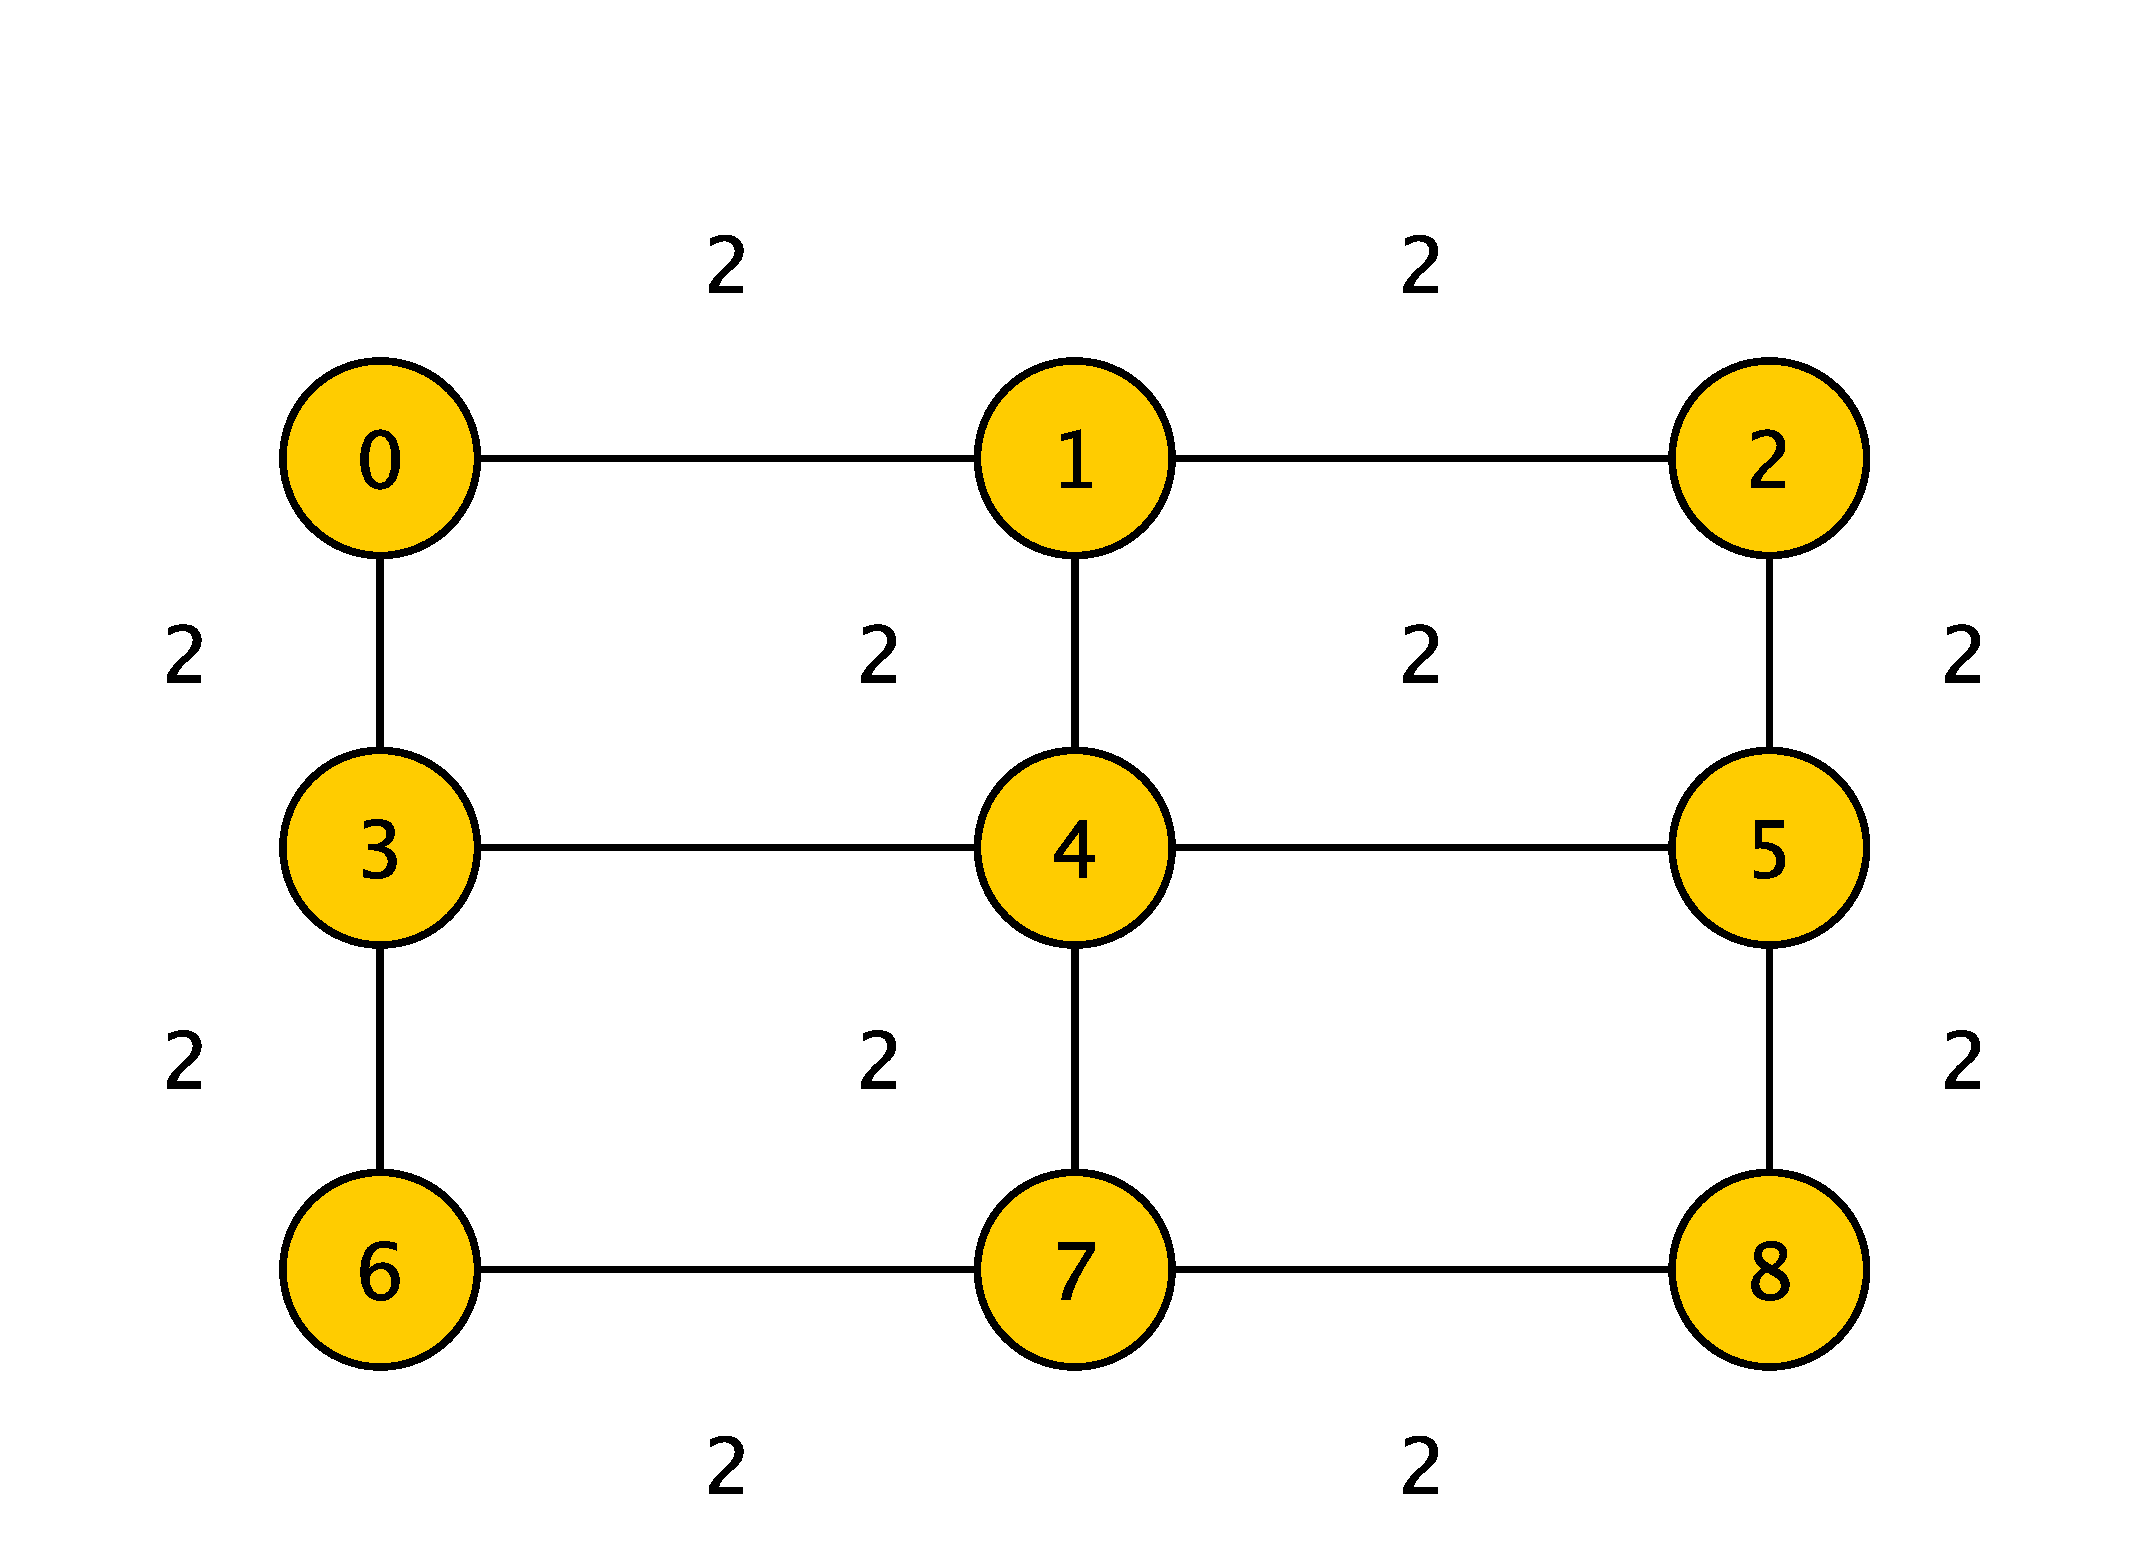
\includegraphics[width=\columnwidth]{img/coarsening.eps}
    \caption{Initial graph}
    \label{img:init_graph}
  \end{figure} 
\end{center}

Figures \ref{img:init_graph} and \ref{img:coarse_graph} illustrate the coarsening phase. During this phase, a sequence of coarser graphs is constructed.\cite{Karypis95parallelmultilevel} A coarser graph is constructed by matching neighbour vertices and then contracting the edges. Thus, the edge between two vertices is collapsed and a multinode consisting of those two vertices is created. Also, the edge-cut of a partition in a coarser graph should be equal to the edge-cut of the same partition in the finer graph.\cite{Karypis:1998:FHQ:305219.305248} This process is achieved in one of two approaches. The first approach consists on finding a random matching and created a multinode with the process described above, while the second approach consists of matching groups of vertices that are highly connected.\cite{Karypis:1998:FHQ:305219.305248}

\begin{center}
  \begin{figure}[htb]
    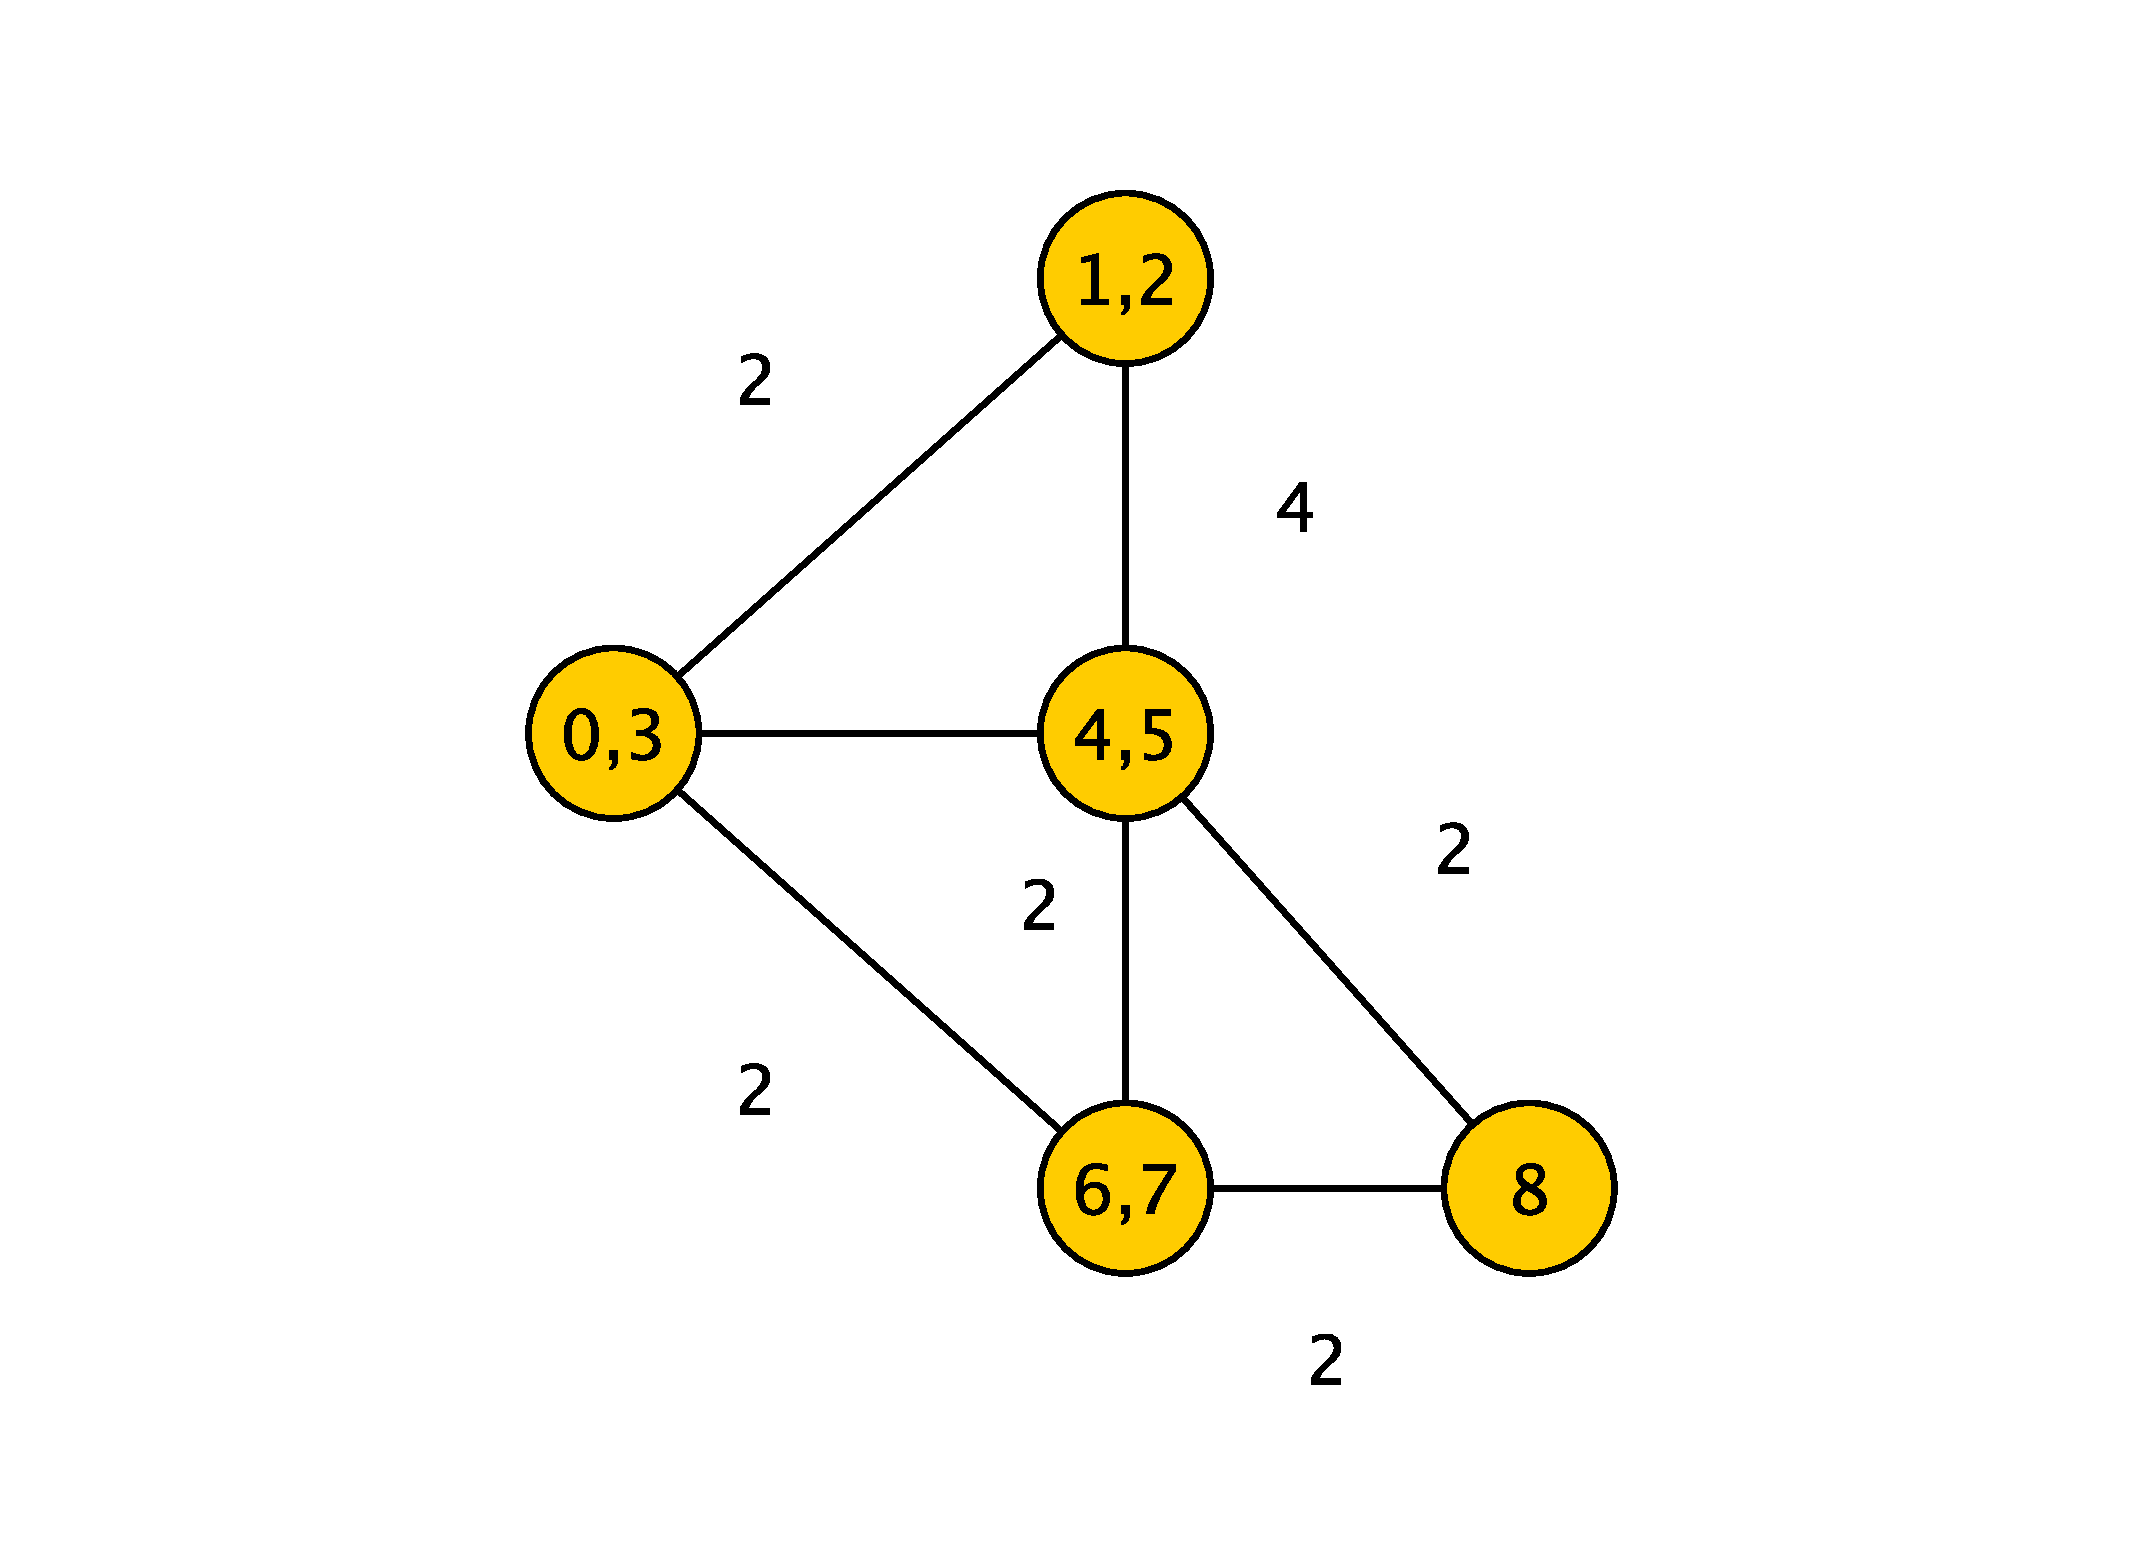
\includegraphics[width=\columnwidth]{img/coarsening2.eps}
    \caption{Coarsened graph}
    \label{img:coarse_graph}
  \end{figure}
\end{center}

Figure \ref{img:part_graph} displays the partitioned graph, this is the next step in the algorithm. To do this, a Greedy Graph Growing (GGGP) algorithm is used.\cite{Karypis:1998:FHQ:305219.305248} The goal of this phase, is to compute a high quality bisection (e.g., small edge-cut) of the coarsened graph such that each part contains roughly half of the vertices and edges of the original graph.
\begin{center}
  \begin{figure}[htb]
    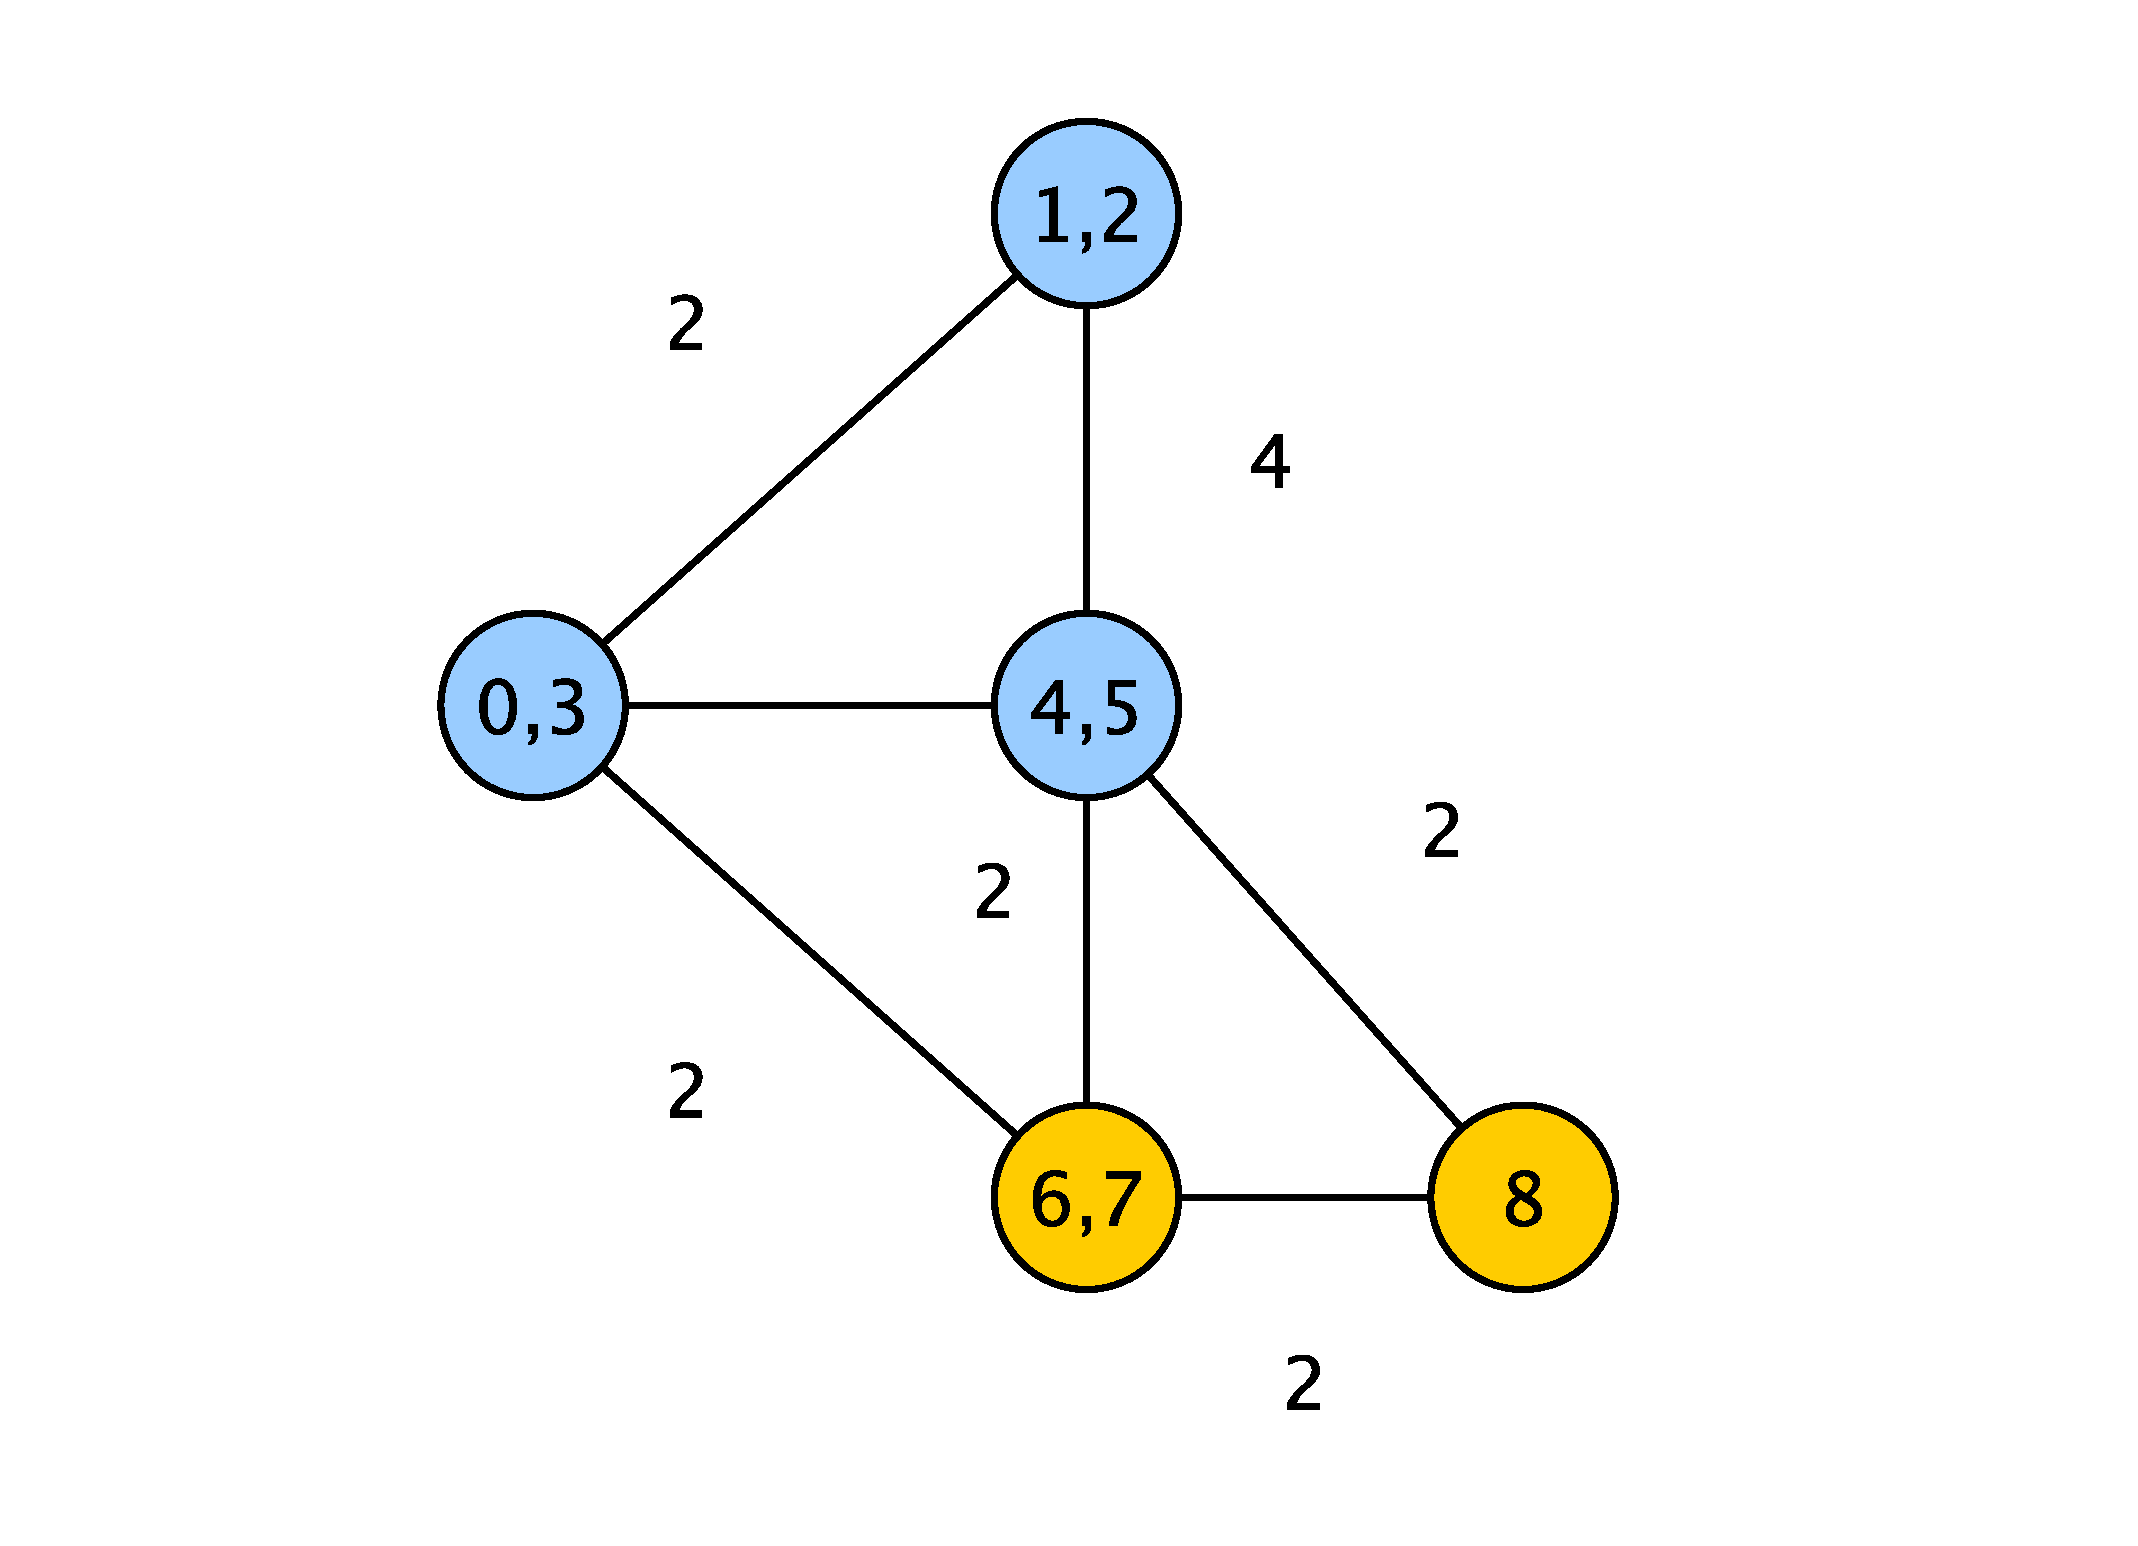
\includegraphics[width=\columnwidth]{img/partition.eps}
    \caption{Partitioned graph}
    \label{img:part_graph}
  \end{figure}
\end{center}

Figure \ref{img:refined_graph} shows the results of the refinement phase. During this stage, the partition of the coarser graph is projected back to the original graph by going through the graphs.\cite{Karypis:1998:FHQ:305219.305248}
Once again, the goal here, is to minimize the edge-cut, however, a good balance in the number of vertices assigned to each partition is also very important. Hence, in this final phase, some algorithms use special heuristics to further improve on the balancing achieved.
\begin{center}
  \begin{figure}[htb]
    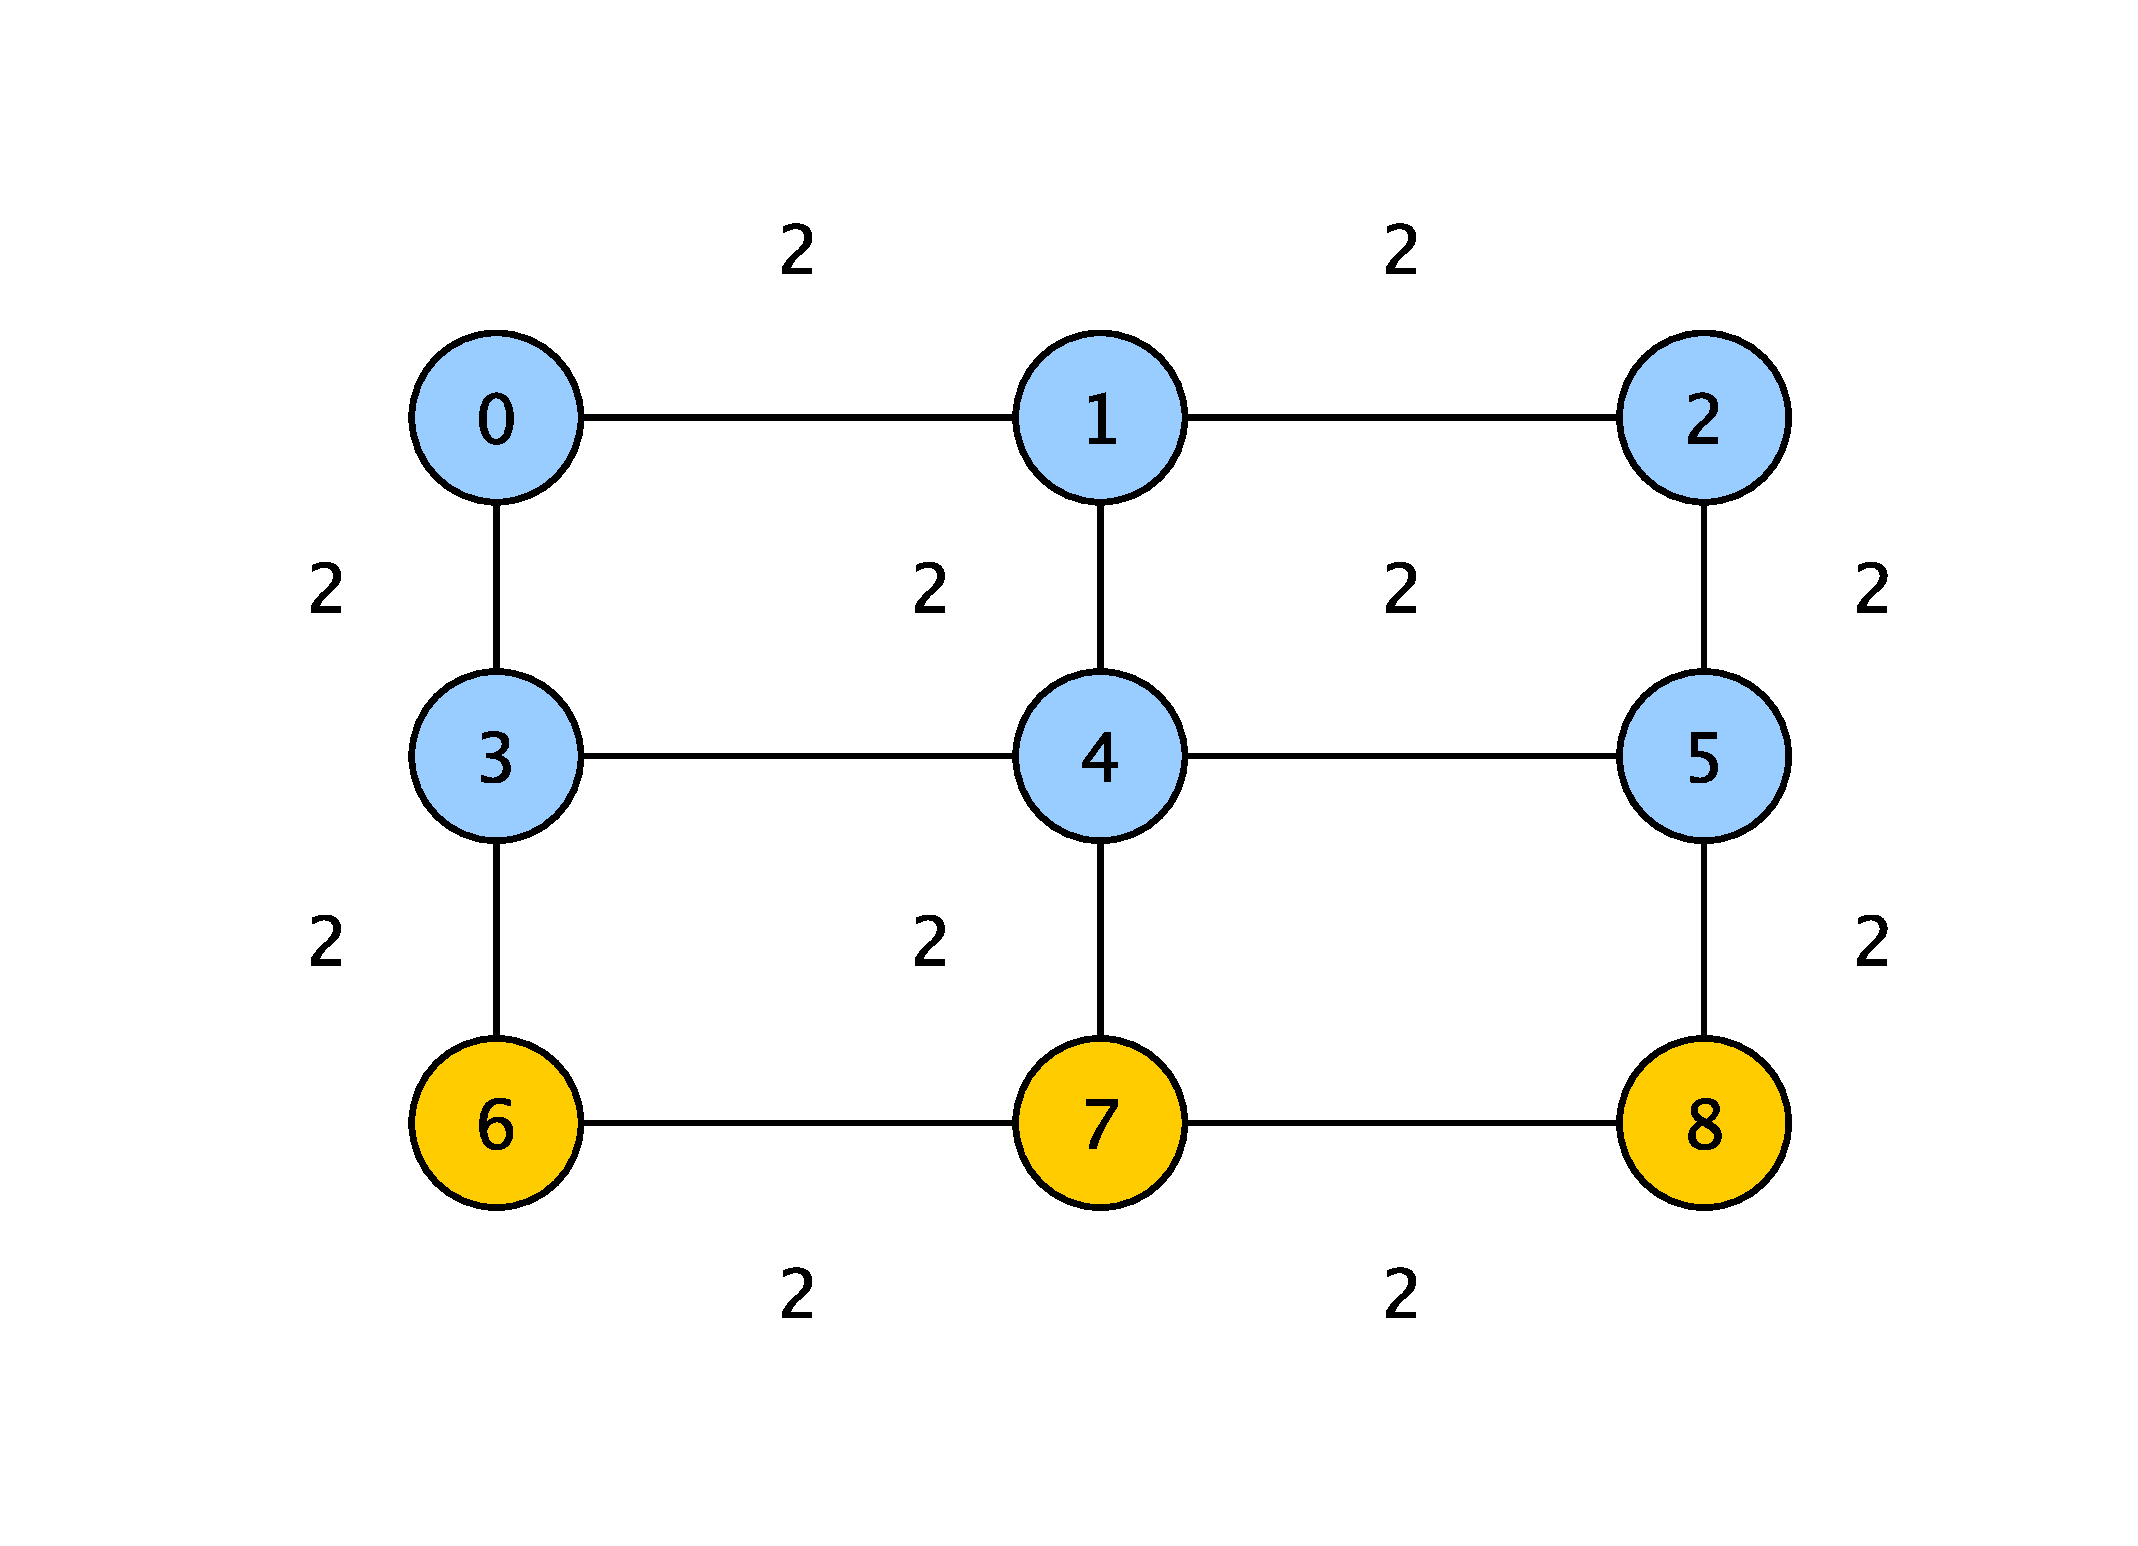
\includegraphics[width=\columnwidth]{img/refinement.eps}
    \caption{Refined graph}
    \label{img:refined_graph} 
  \end{figure}
\end{center}


%-----------------------------------------------------------------------------
% System characteristics
%-----------------------------------------------------------------------------

\section{System characteristics}
\label{sec:sys_char}

The measurements were performed in both Stampede's hosts and
co-processors.
The hosts are comprised of dual Intel Xeon E5-2680, while the
co-processors are the new Intel Xeon Phi with 61 cores. Their
characteristics are presented in the following tables.

\begin{table}[H]
\centering
\footnotesize
\begin{tabular}{| c | c |}\hline
Manufacturer & Intel\\ \hline
Model & Xeon E5-2680\\ \hline
$\mu$Arch & Sandy Bridge\\ \hline
Clock freq & 2.70 GHz\\ \hline
\#CPUs (sockets) & 2 \\ \hline
\#Cores/CPU & 8\\ \hline
\#Thread/Core & 1\\ \hline
L1 cache size/core & 32 KB\\ \hline
L2 cache size/core & 256 KB\\ \hline
L3 shared cache size/CPU & 20 MB\\ \hline
Main Memory/CPU & 16 GB\\ \hline
Vector width & 256 bits (AVX)\\ \hline
\end{tabular}
\label{tab:host_stampede}
\caption{Intel Xeon E5-2680}
\end{table}

\begin{table}[H]
\centering
\footnotesize
\begin{tabular}{| c | c |}\hline
Manufacturer & Intel\\ \hline
Model & Xeon Phi SE10P\\ \hline
$\mu$Arch & Many Integrated Cores - MIC\\ \hline
Clock freq & 1.1 GHz\\ \hline
\#CPUs (sockets) & 1 \\ \hline
\#Cores/CPU & 61\\ \hline
\#Thread/Core & 4\\ \hline
L1 cache size/core & 32KB\\ \hline
L2 cache size/core & 512 KB\\ \hline
Main Memory/CPU & 8 GB\\ \hline
Vector width & 512 bits\\ \hline
\end{tabular}
\label{tab:mic}
\caption{Intel Xeon Phi}
\end{table}

As can be seen, the Intel Xeon Phi only has 8 GB of memory, thereby
limiting large input graphs to run with GMetis. Therefore, all
measurements were done with the USA-W roadmap, which is the largest graph
that still fits in memory. This graph contains 6262104 nodes and 15248146 edges.

%-----------------------------------------------------------------------------
% Xeon Phi
%-----------------------------------------------------------------------------

Apart from the characteristics showed in table \ref{tab:mic}, there are
others that should be mentioned. Each core contains a in-order dual-issue pipeline which can issue two instructions from the same hardware thread
per clock cycle. However, the front-end of the pipeline does not issue
instructions from the same hardware thread in consecutive cycles.\cite{Cepeda:PhiPerformance}

This means that the maximum issue rate is only attainable with at least
2 threads per core while the other threads have the purpose of hiding
pipeline stalls due to memory latency.

The fact that the pipeline issues in-order instructions increases
memory related problems. %FIXME: Pode-se dar o exemplo do andrew

\begin{center}
\begin{figure}[htb]
    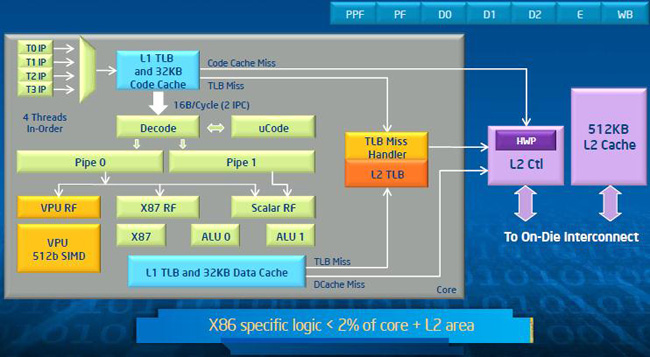
\includegraphics[width=\columnwidth]{img/phi_arch.jpg}
    \caption{Xeon Phi $\mu$Arch}
    \label{img:phi_arch}
\end{figure}
\end{center}


%-----------------------------------------------------------------------------
% Metis %FIXME: Pôr isto mais acima?
%-----------------------------------------------------------------------------

\section{Metis}
\label{sec:metis}


The version of Metis we used to perform measurement was 5.1.0

%-----------------------------------------------------------------------------
% Mt-metis
%-----------------------------------------------------------------------------

\section{Mt-metis}
\label{sec:mt-metis}

The next plot shows the scalability of Mt-metis on Xeon Phi\footnote{All measurements were taken using version 0.1 of mt-metis.}. 
Despite the large number of measurements taken, results shows spikes when running mt-metis with a certain number of partitions. We can see that
mt-metis scales up to 28 threads, declining rapidly for more than 60 threads. 
This is mainly due to the clustering and refinement stages, since, as we can see from the figure, the coarsening stage is relatively well behaved. 
The behaviour of the refinement phase is somewhat to be expected, since, with the higher number of threads, as conflicts arise, it is expected for its running time to go up.
The problem here, is the Partitioning (Clustering) phase, since its behaviour in unpredictable as the number of threads go beyond 60. We believe the explanation for this behaviour lies the Xeon Phi's architecture, since, as explained above, the maximum issue rate is 2. Combining this with a higher number of threads, the amount of stalls and ensuing context switches is expected to go up. This can be especially bad if the application has a lot of memory random memory accesses, which is the case.  

\begin{center}
\begin{figure}[htb]
    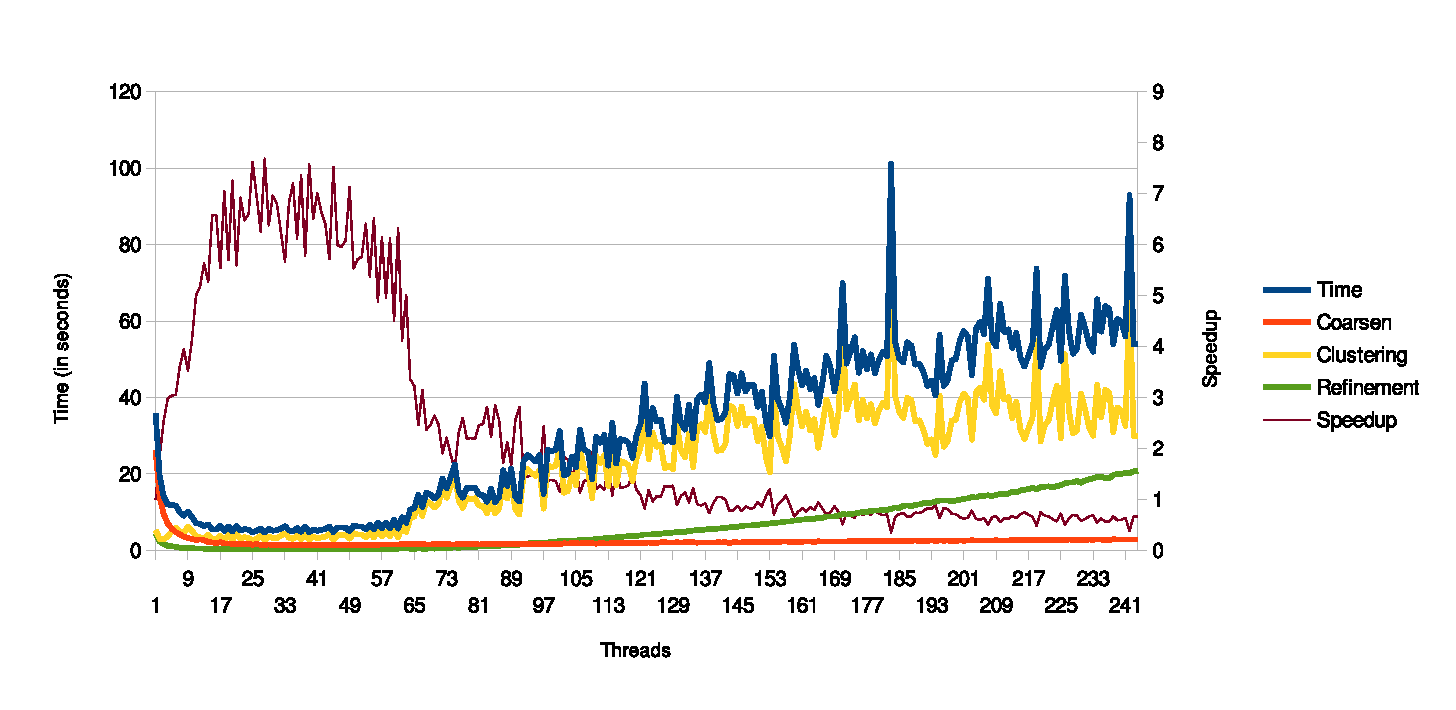
\includegraphics[width=\columnwidth]{img/mtmetis128.eps}
    \caption{Mt-metis - 128 partitions}
    \label{img:mtmetis128}
\end{figure}
\end{center}


%-----------------------------------------------------------------------------
% GMetis and Galois Framework
%-----------------------------------------------------------------------------

\section{GMetis and the Galois Framework} %FIXME: Mudar o nome do titulo
\label{sec:GMetis}

\begin{center}
\begin{figure}[htb]
    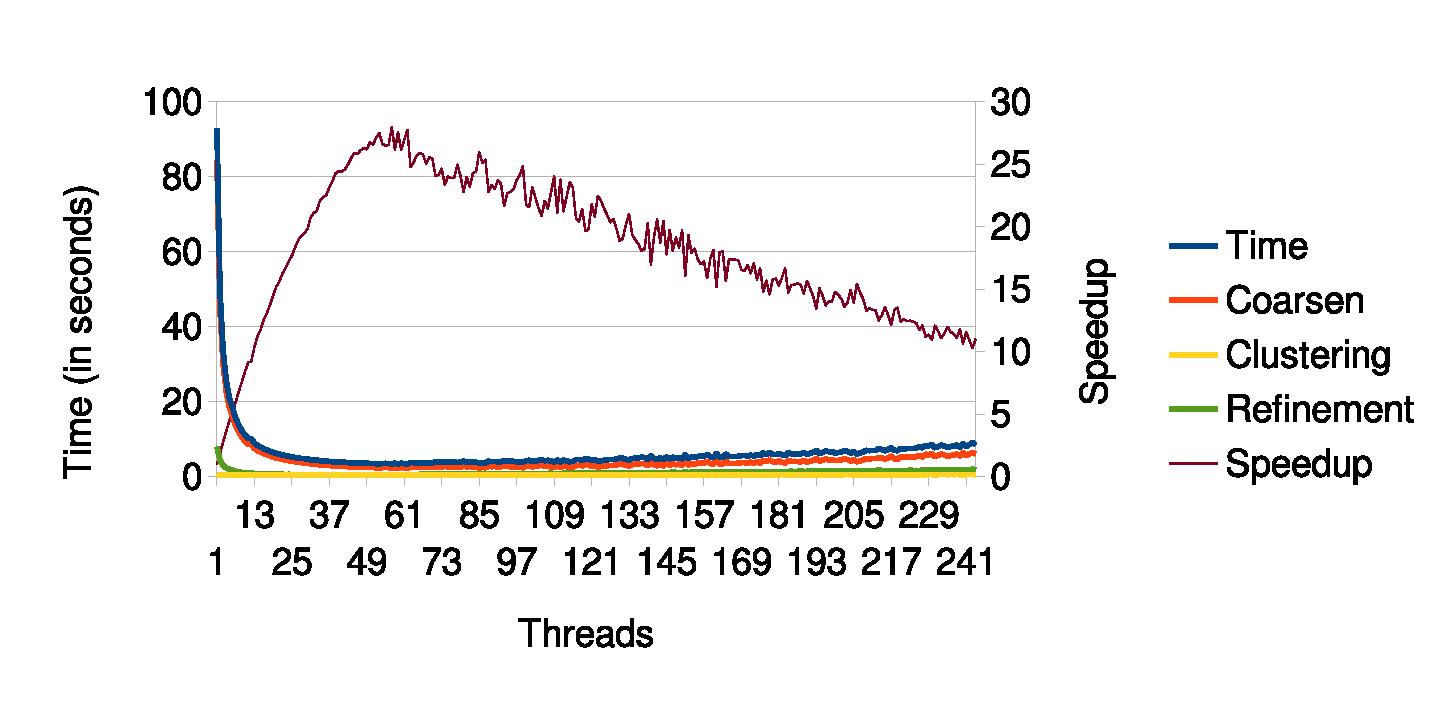
\includegraphics[width=\columnwidth]{img/gmetis128.eps}
    \caption{GMetis - 128 partitions}
    \label{gmetis128}
\end{figure}
\end{center}

This figure shows the scalability of gmetis on Xeon Phi over the runtime
with one thread. This example is for 128 partition, but we did
measurements for different number of partitions, such as 16 and 1024. All
of them have a similar behaviour.


%-----------------------------------------------------------------------------
% Enhancements
%-----------------------------------------------------------------------------
\subsection{Enhancements}

Throughout this month, we did some modifications to improve
\textit{GMetis}' performance. We started by experimenting with how the package mapping
is done internally by the \textit{Galois} framework.

\textit{Galois} has support for \textit{NUMA} systems, thus, this means that
it take advantage of different sockets (packets in Galois terminology) simultaneously.

Before an application starts running, \textit{Galois} parses the
cpuinfo file located in "/proc/cpuinfo" to create its mapping, which means that each socket
corresponds to a package, or rather, all the cores in a socket belong to the same package.
This means that \textit{Galois} was assigning a package to the entire MIC co-processor, since it has 60 usable cores in the same "package".

%TODO: Talvez cagar leis sobre worklists bem como packages e para que
%servem, nomeadamente, loadbalancing
This is especially bad, since the \textit{Galois} framework uses a sort of work stealing mechanism inside each package. It works by assigning a master thread in each package, then each thread inside a package can steal work from another inside the same package. In case of aborts, the work is pushed to a stack in the master thread, if it aborts when that master thread pops from the stack, then the work is pushed in another packet's stack. In the MIC, since there is only one packet, this means that all 244 threads were stealing work from each other. Hence, worst case scenario, the code is run serially. 

Also, it should be noted that, since \textit{Galois} was not prepared to deal with a processor that supports more than two-way hyperthreading, when using different thread values, some processor cores could have four threads running, while others only one (default mapping).

We changed that, by assigning each hyperthread to its respective core id (which would make a packet).
Another reason for this change is so that the mapping could be
the most balanced possible (load balanced mapping)\footnote{Although the Xeon Phi contains 61 cores, it should be noted that the
operating system also needs to run. Therefore, only 60 cores may be
available for computations tasks.}, for instance,
when running the application with 121 threads, with the default mapping,
the first 20 cores will run with four threads while the others will only
run with one thread. With the load balance mapping, only the last core
will run one thread, while the others will run 2 threads. However, this did not achieve any considerable improvements. We also tried assigning each thread to a packet in a round-robin fashion (dense package mapping), but that proved to be ineffective as well.

Unfortunately, Intel VTune only has support for Stampede's hosts, and
not for the co-processor. Although, Intel states that profiling and
improving an application on the host gives similar improvements on MIC,
profiling support for the MIC architecture on \textit{Stampede} would be
welcome, as there are key differences in the architectures.

Thereby, we profiled the application with the help of simple timers as
well as PAPI, and we found the most time consuming function, which is
findMatching. This function iterates through the graph's nodes, trying
to match each node with one available neighbor.

This function is part of the \textit{Coarsening} phase, together with
the \textit{CreateCorseEdge}.
The coarsening phase as the objective of coarsening a graph so it can be
more easily partitioned. This is done mainly in two phases. The first,
findMatching, matches nodes that have not been matched yet, and creates
a "supernode" for each pair of matched nodes. The
\textit{CreateCorseEdge} creates the edges between "supernodes", merging
edges that are shared between the two nodes of the supernode and their
common neighbors.

%TODO: Falar um pouco mais sobre isso, dizer que depois ficam matched, e
%que por isso, alguns nós podem ficar sozinhos (pk nao têm nodos livres
%para fazer match).

There are different ways to match the graph's nodes. The ones used are
"Heavy Weight Match" and "Random Match". The first iterates through each
node and matches them with the neighbor whose shared edge has the most
weight. The second matches each node with the first neighbor node that
has not been matched yet.

Previously, these were used separately, i.e., only one of them was
used in the application. Using the two combined proved to be a better
solution, as the performance improved, and the edge-cut remained the
same. Random Match is used in the first two iterations of the coarsening
phase. This improved runtime because, RM computes faster, as it does not
need to iterate through all neighbors when there is a node that has not
been matched. The algorithm is used only on the first two iterations
because the graph is larger on these iterations, and using RM instead of
HEM on small graphs did not prove to be any faster and can actually worsen
edge-cut.

%Due to incompatibilities of some C++11 functions, we tried to compile
%the code with x86\_64-k1om-linux-gcc, which is gcc with MIC support.
%TODO: Falar do gcc e do icc
A deeper look into the assembly code generated by the two compilers
shows that gcc does not introduce prefetch instructions (even when using
\_\_builtin\_prefetch) as opposed to icc that prefetches. The results,
however, runtime differences are minimal.

We also did some tests with different worklist schedulers provided by
Galois. AltChunkedLIFO<8> was the fastest and it is actually the most
scalable one.

Some extra measurements allowed us to find that with 45-50 partitions
, GMetis start to run faster than mt-metis.


%-----------------------------------------------------------------------------
% Final results
%-----------------------------------------------------------------------------

The following figure compares the runtime of each application. Metis was
executed in one of the Xeon Phi's core, while mt-metis and gmetis were executed
for each number of threads, for the three partitions number. For those, the best execution time was
chosen. The time of the sequential metis is included to see how much
speedup both mt-metis and gmetis obtains for each partition number. 
We can see that for 16 partitions, mt-metis run faster than gmetis,
achieving a total speedup of 24x as opposed to the 17x of gmetis.
For the other partitions, gmetis is actually faster, achieving a total
speedup of 17x and 11x for 128 and 1024 partitions respectively.

%mt-metis128 com melhor tempo com 28 threads
%gmetis128 com melhor tempo com 70 threads


%FIXME: Dizer com que número de threads se atingiu o melhor tempo?
%FIXME: Qual das duas imagens se usa??????

\begin{center}
\begin{figure}[htb]
    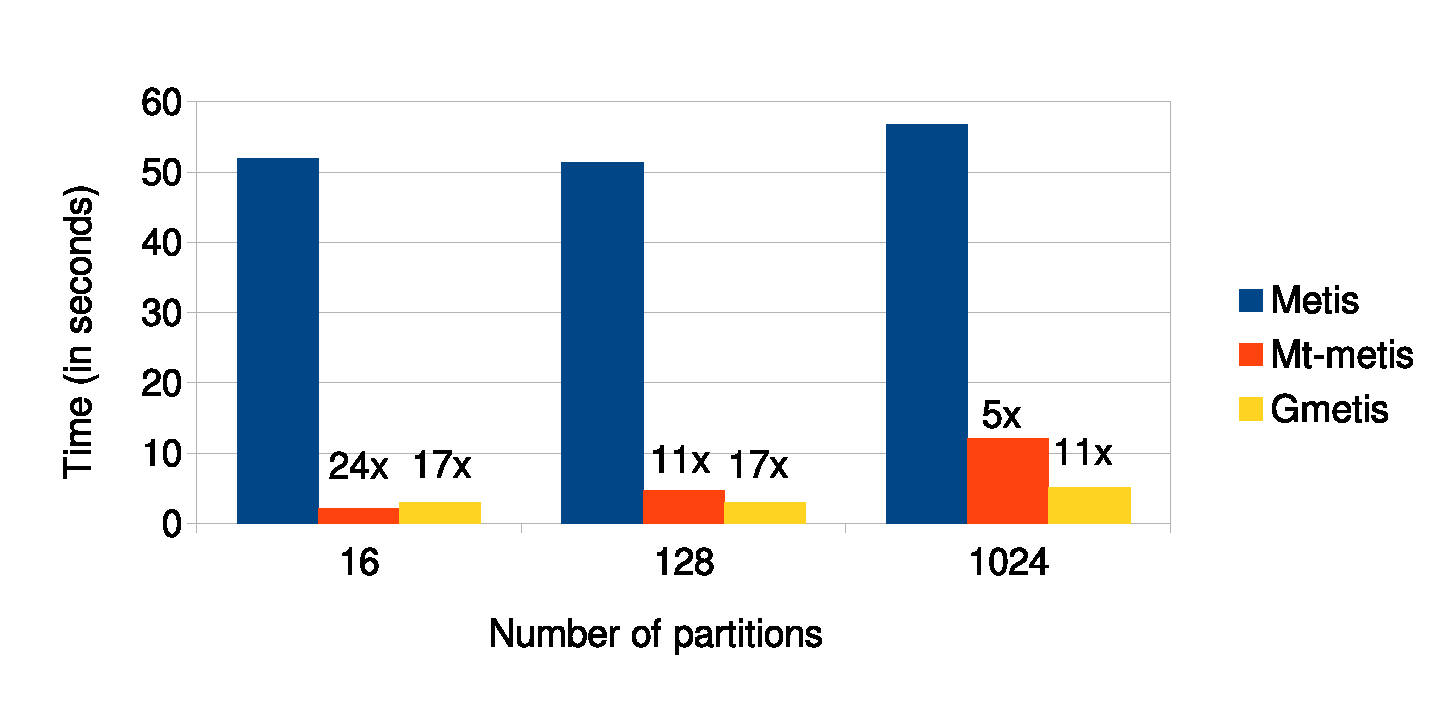
\includegraphics[width=\columnwidth]{img/comparison3.eps}
    \caption{Comparison}
    \label{img:comparison3}
\end{figure}
\end{center}

\begin{center}
\begin{figure}[htb]
    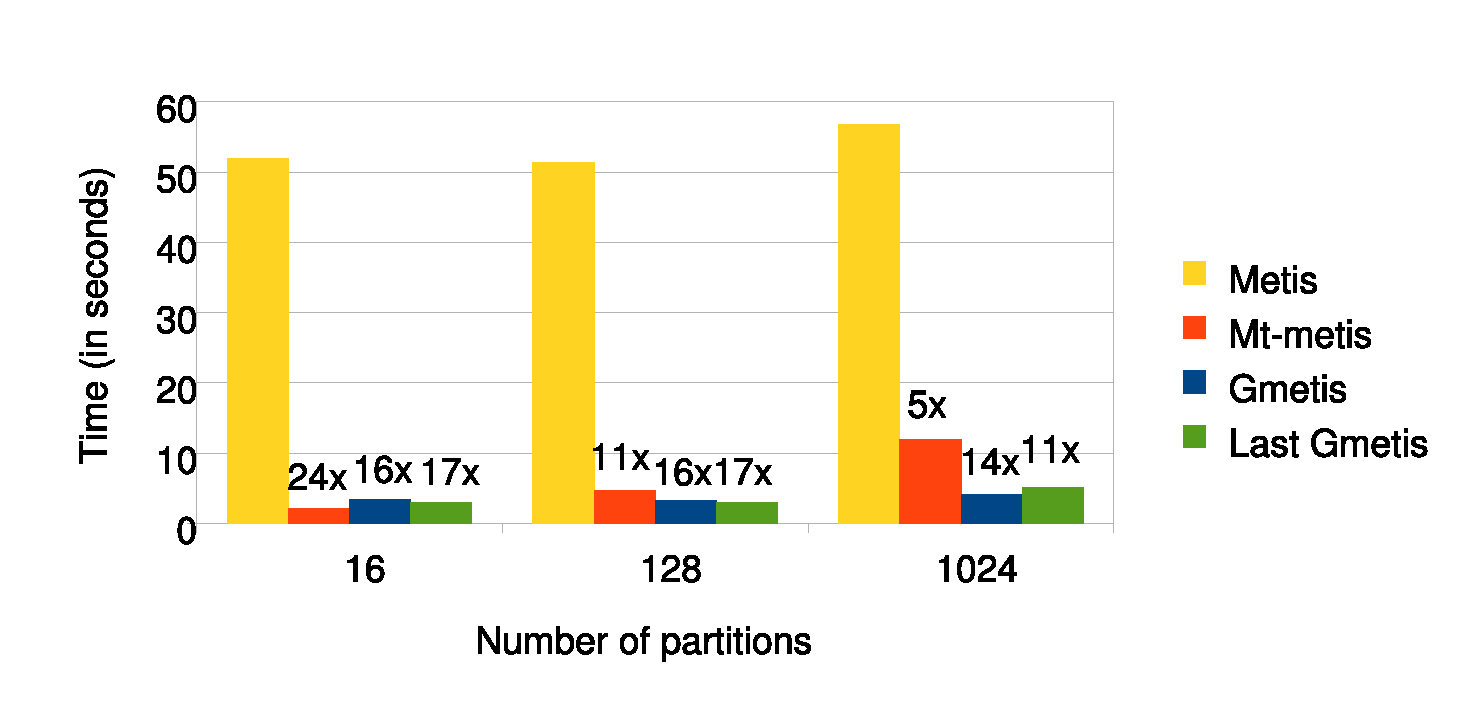
\includegraphics[width=\columnwidth]{img/comparison4.eps}
    \caption{Comparison}
    \label{img:comparison4}
\end{figure}
\end{center}

%TODO: Falar que o metis tenta obter partições o mais balanceadas
%possiveis na parte da introdução
As previously stated, the objective of \textit{Metis} is to partition a graph in a way
that the partitions are balanced and the edge-cut between them is the smallest
possible. For this last metric, GMetis performs worse. According to the
measurements made on figure~\ref{img:edgecut}, \textit{GMetis} edge-cut is
always more than two times higher than metis and mt-metis. The openMP
version of metis performs a little bit worse than its original version.

\begin{center}
\begin{figure}[htb]
    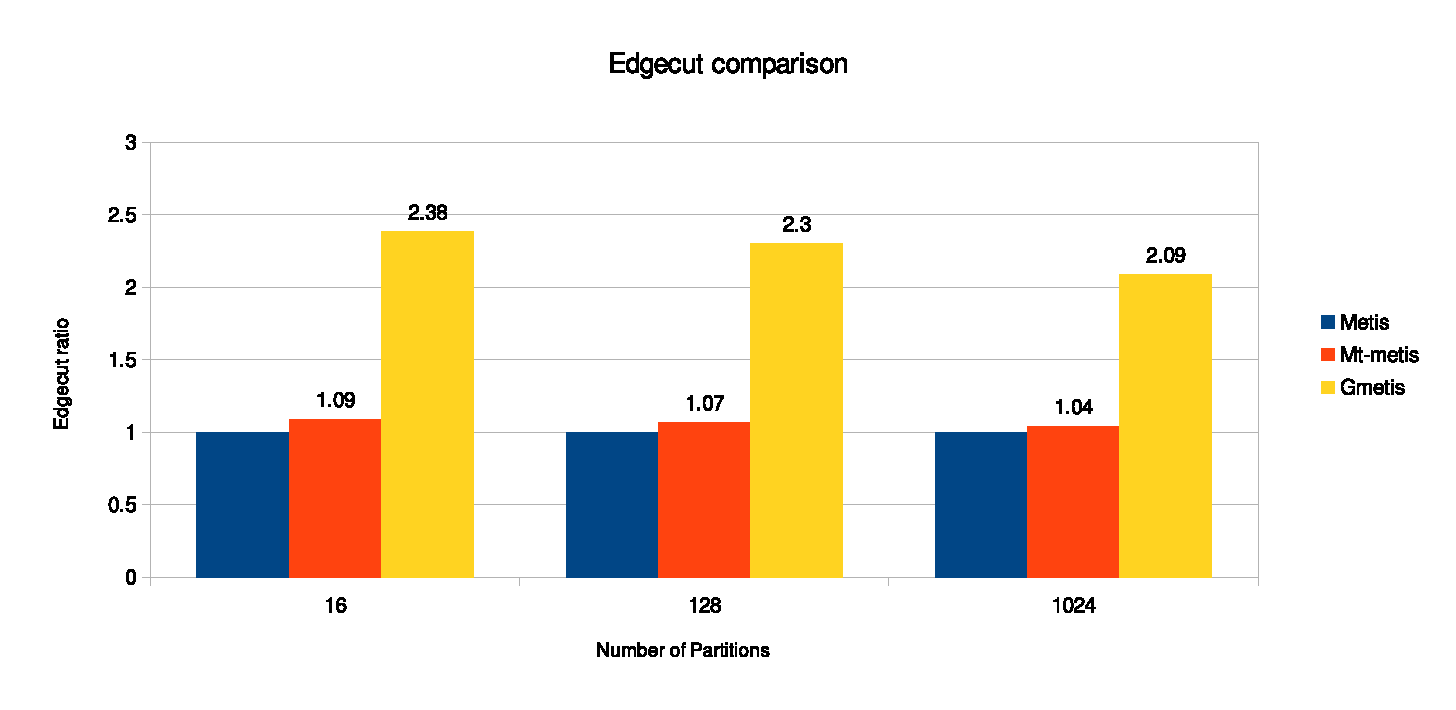
\includegraphics[width=\columnwidth]{img/edgecut.eps}
    \caption{Comparison}
    \label{img:edgecut}
\end{figure}
\end{center}


%-----------------------------------------------------------------------------
% Conclusion
%-----------------------------------------------------------------------------

\section{Conclusion}
\label{sec:conc}
Results showed that both \textit{Metis} and \textit{Mt-metis} have
better edge-cut than \textit{Gmetis}. However, Gmetis's runtime is lower
for a high number of partitions.

%FIXME: Adicionar o número de partições em que o GMetis passa a ser mais
%rápido

Xeon Phi provides a theoretical performance of 2112 GFlop/sec for double
precision arithmetic and 1056 GFlops/sec for single precision
arithmetic. This values comprises the use of 60 cores since one core is
necessary to perform operating system operations.


%-----------------------------------------------------------------------------
% Bibliography
%-----------------------------------------------------------------------------

\bibliographystyle{plain}
\bibliography{references}


\end{document}
